%\documentclass[nototal]{beamer}
\documentclass[nototal,handout]{beamer}

% This file is a solution template for:

% - Talk at a conference/colloquium.
% - Talk length is about 20min.
% - Style is ornate.


%
% In principle, this file can be redistributed and/or modified under
% the terms of the GNU Public License, version 2.
%
% However, this file is supposed to be a template to be modified
% for your own needs. For this reason, if you use this file as a
% template and not specifically distribute it as part of a another
% package/program, I grant the extra permission to freely copy and
% modify this file as you see fit and even to delete this copyright
% notice. 


\mode<presentation>
{
  %\usetheme{Madrid}
 \usetheme{Boadilla}
  % or ...

  \setbeamercovered{transparent}
  % or whatever (possibly just delete it)
}

\usepackage{verbatim}
\usepackage[english]{babel}
% or whatever

\usepackage[latin1]{inputenc}
% or whatever

%\usepackage{bar}
\usepackage{times}
\usepackage[T1]{fontenc}
% Or whatever. Note that the encoding and the font should match. If T1
% does not look nice, try deleting the line with the fontenc.
\usepackage{graphicx} %sjr added
\graphicspath{{figures/}}
\usepackage{hyperref}

\author{\textsc{Sergio Rey}}
\institute[COGS]{\textbf{GEOG 384}\\\textbf{Spatial Data Analysis}\\Center for
  Open Geographical Science\\Department
  of Geography\\San Diego State University\\Fall 2023}
\title[Geostatistics Basics]{Geostatistics Basics}
\subtitle{}
\date[GEOG 385]{}


% - Either use conference name or its abbreviation.
% - Not really informative to the audience, more for people (including
%   yourself) who are reading the slides online

% This is only inserted into the PDF information catalog. Can be left
% out. 



% If you have a file called "university-logo-filename.xxx", where xxx
% is a graphic format that can be processed by latex or pdflatex,
% resp., then you can add a logo as follows:

% \pgfdeclareimage[height=0.5cm]{university-logo}{university-logo-filename}
% \logo{\pgfuseimage{university-logo}}



% Delete this, if you do not want the table of contents to pop up at
% the beginning of each subsection:
\AtBeginSubsection[]
{
  \begin{frame}<beamer>
    \frametitle{Outline}
    \tableofcontents[currentsection,currentsubsection]
  \end{frame}
}


% If you wish to uncover everything in a step-wise fashion, uncomment
% the following command: 

%\beamerdefaultoverlayspecification{<+->}


\begin{document}

\begin{frame}
  \titlepage
\end{frame}

\begin{frame}
  \frametitle{Outline}
  \tableofcontents
  % You might wish to add the option [pausesections]
\end{frame}


% Structuring a talk is a difficult task and the following structure
% may not be suitable. Here are some rules that apply for this
% solution: 

% - Exactly two or three sections (other than the summary).
% - At *most* three subsections per section.
% - Talk about 30s to 2min per frame. So there should be between about
%   15 and 30 frames, all told.

% - A conference audience is likely to know very little of what you
%   are going to talk about. So *simplify*!
% - In a 20min talk, getting the main ideas across is hard
%   enough. Leave out details, even if it means being less precise than
%   you think necessary.
% - If you omit details that are vital to the proof/implementation,
%   just say so once. Everybody will be happy with that.
\section{Geostatistical Perspective}
\subsection{Spatial Random Field}
\begin{frame}[<+->]
  \frametitle{Spatial Random Field}
  \begin{block}{Continuous Spatial Process}
    \begin{equation}
    \left \{ Z(s): s \in D \right \}
    \end{equation}
    \begin{itemize}
      \item $s$ is spatial index, continuous in $R^2$ $(R^3)$
      \item Sample of spatial locations
	\begin{itemize}
	  \item $\left \{ s_1,s_2,\ldots,s_n \right\}:$ sample locations
	  \item $\left \{ Z(s_1),Z(s_2),\ldots,Z(s_n) \right\}:$ random
	    variable at sample locations
	\end{itemize}
    \end{itemize}
   \end{block}
 \end{frame}
\begin{frame}[<+->]
  \frametitle{Geostatistical Data}
  \begin{block}{Spatial Domain: $D$ }
    \begin{itemize}
      \item A continuous and fixed set.
      \item Meaning $Z(s)$ can be observed everywhere within $D$.
      \item Between any two sample locations $s_i$ and $s_j$ you can
	theoretically place an infinite number of other samples.
      \item By fixed: the points in $D$ are non-stochastic
    \end{itemize}
   \end{block}
\begin{block}{Continuous Variation}
    \begin{itemize}
      \item Because of the continuity of $D$
      \item Geostatistical data is referred to as ``spatial data with
	continuous variation.''
      \item Continuity is associated with $D$.
      \item Attribute $Z$ may, or may not, be continuous.
    \end{itemize}
   \end{block}
 \end{frame}
 \begin{frame}
   \frametitle{Geostatistical Data: Rainfall in Parana State Brazil}
   \begin{center}
     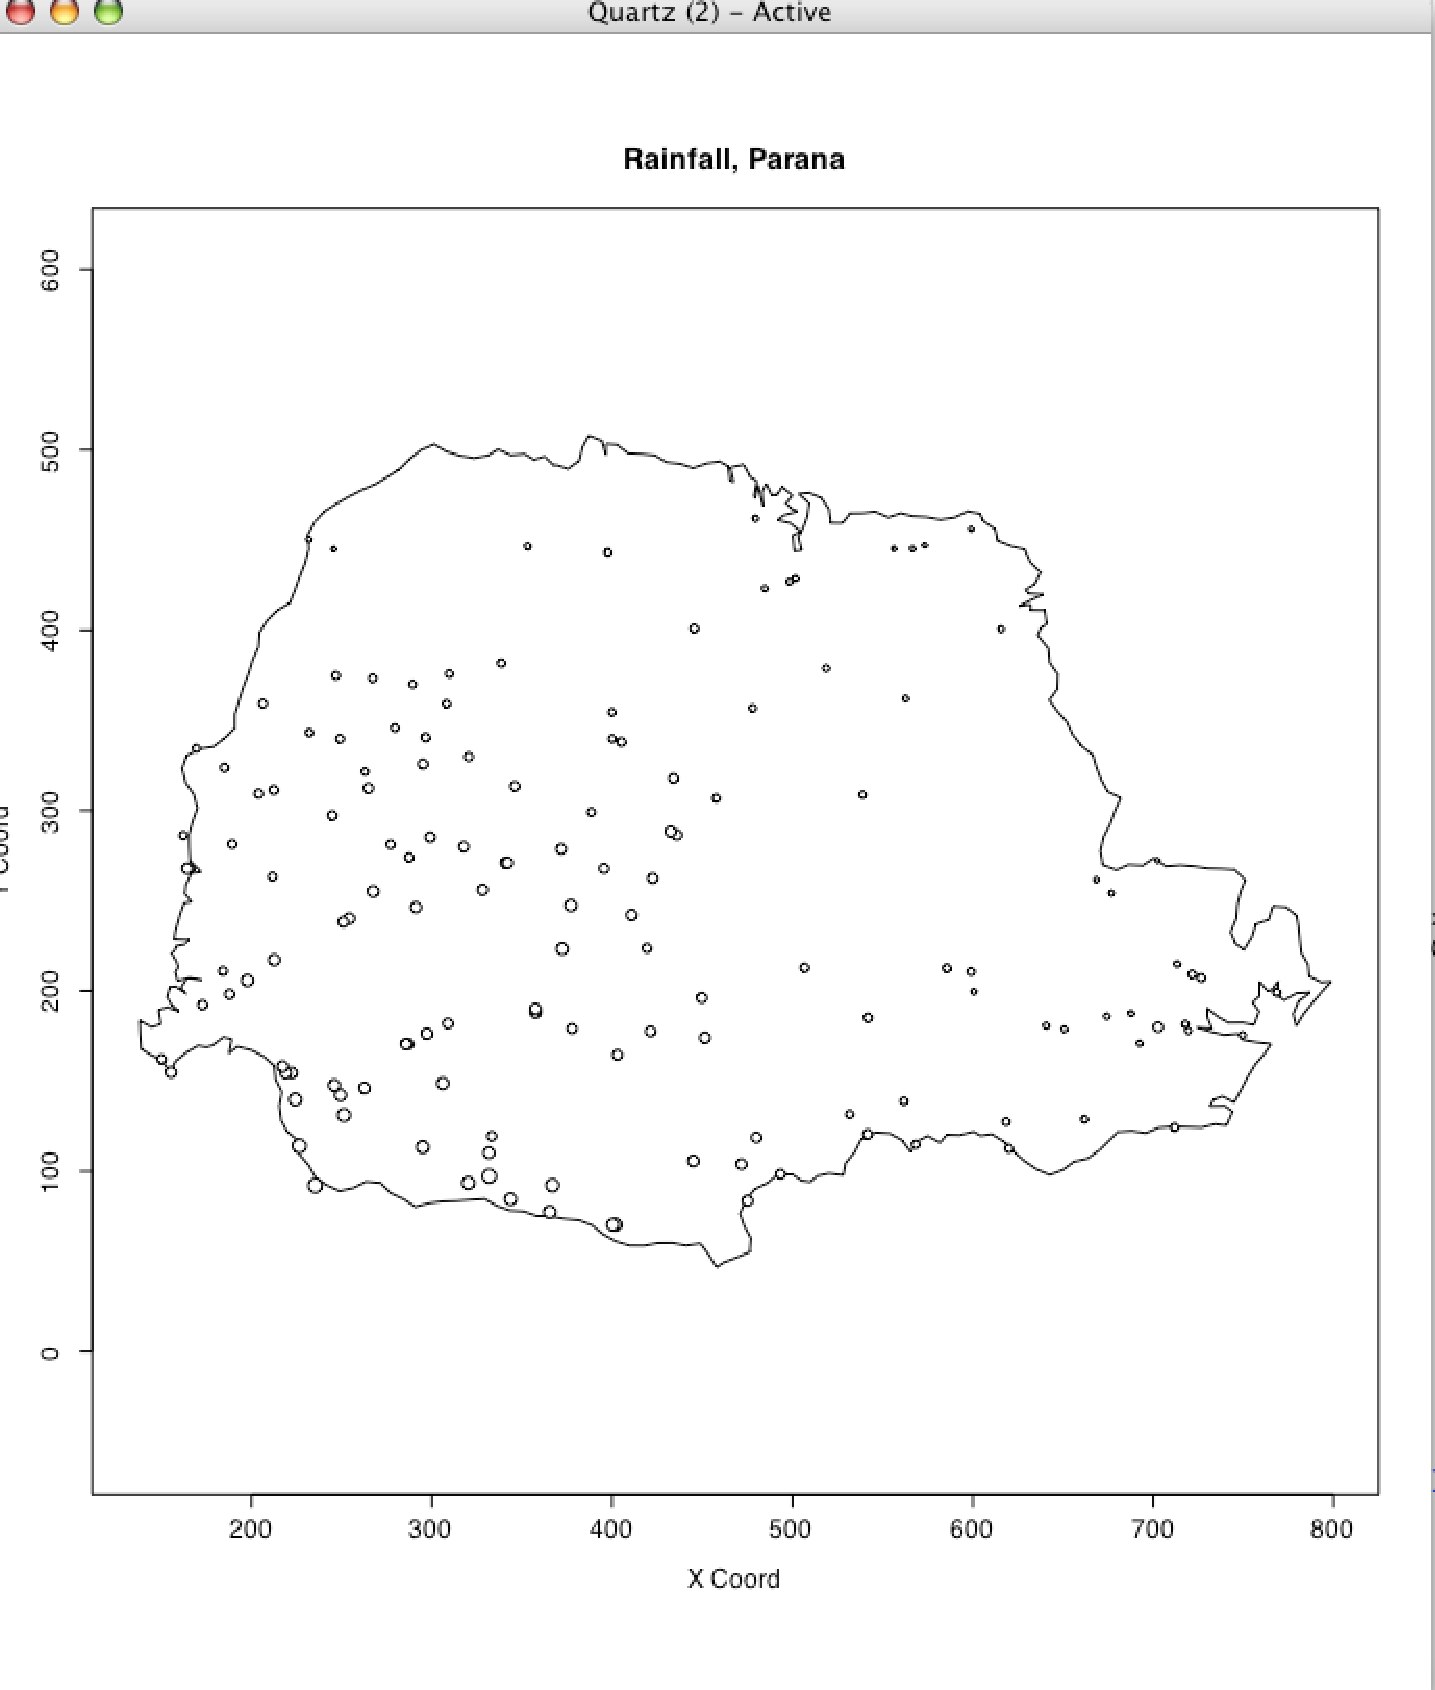
\includegraphics[width=.65\linewidth]{rainfall.pdf}
   \end{center}
 \end{frame}
 \begin{frame}[<+->]
   \frametitle{Geostatistical Data}
   \begin{block}{Continuous variation}
     \begin{itemize}
       \item Potentially measurable anywhere in $D$
       \item Impossible to sample $D$ exhaustively
     \end{itemize}
    \end{block}
\begin{block}{Reconstruction of the surface from observed sites}
     \begin{itemize}
       \item Tessellation based methods
       \item Interpolation
       \item Kriging
     \end{itemize}
    \end{block}
  \end{frame}
  \begin{frame}
    \frametitle{Surface Reconstruction: Example\footnote{From Goovaerts, P.
    (1999)``Performance comparison of geostatistical algorithms for
    incorporating elevation into the mapping of precipitation''.
    \emph{Geocomputation '99}.}}
    \begin{center}
      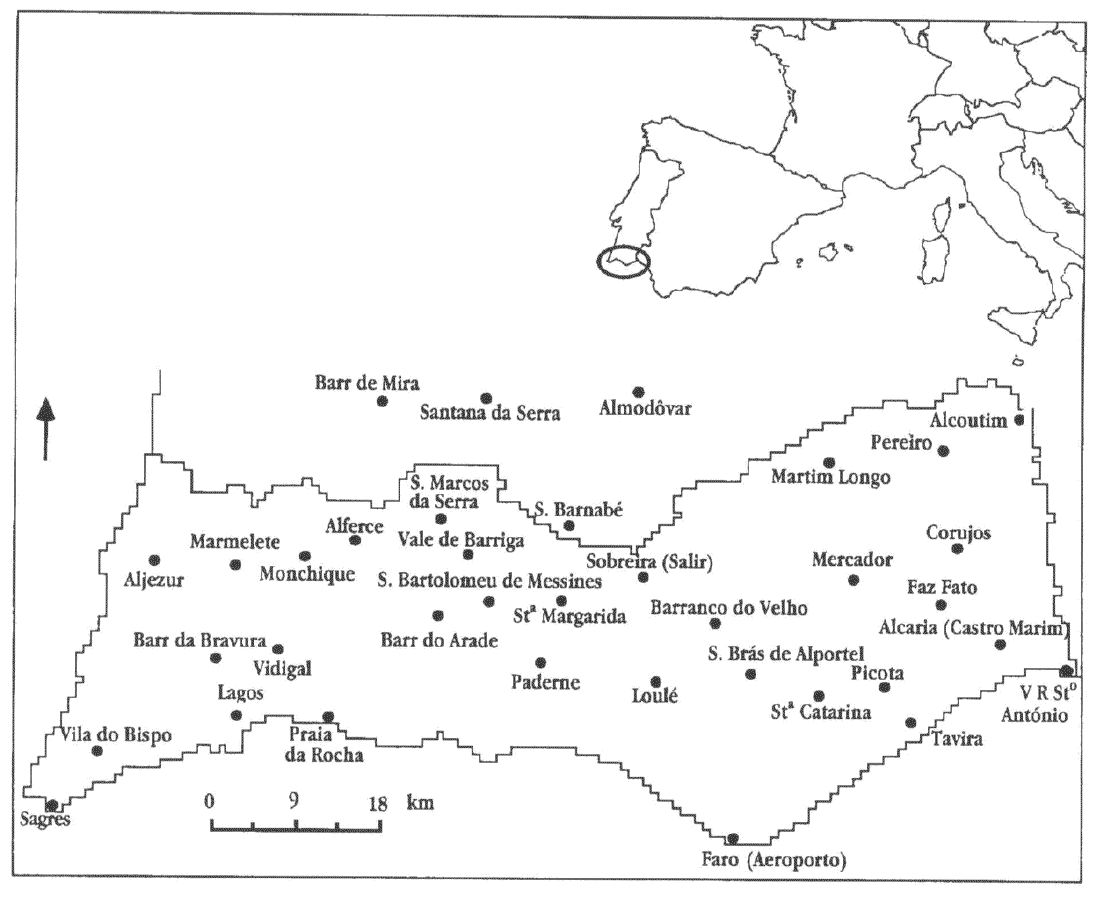
\includegraphics[width=.65\linewidth]{pg1.jpg}
    \end{center}
  \end{frame}
\begin{frame}
    \frametitle{Surface Reconstruction: Tessellation Based Method}
    \begin{center}
      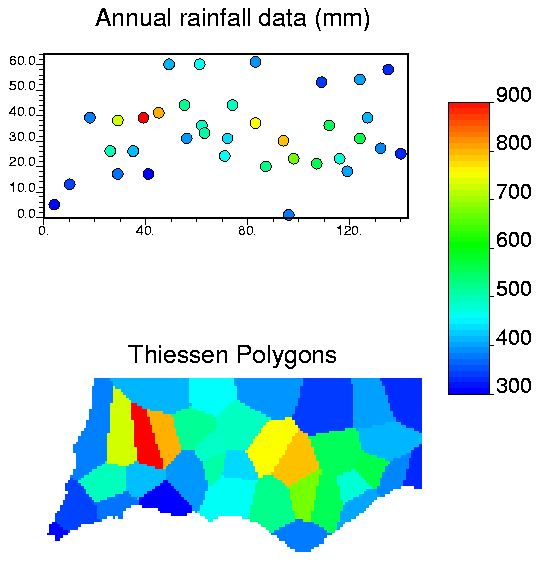
\includegraphics[width=.65\linewidth]{pg2.jpg}
    \end{center}
  \end{frame}
\begin{frame}
    \frametitle{Surface Reconstruction: Spatial Interpolation}
    \begin{center}
      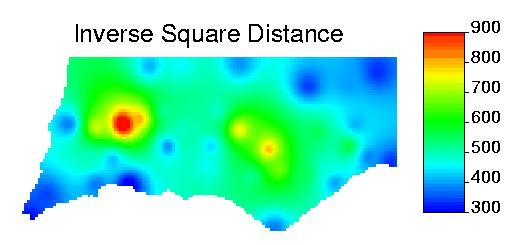
\includegraphics[width=.65\linewidth]{pg3.jpg}
    \end{center}
  \end{frame}
\begin{frame}
    \frametitle{Surface Reconstruction: Kriging}
    \begin{center}
      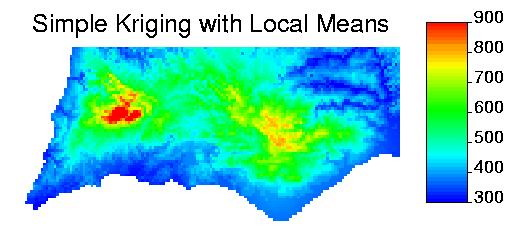
\includegraphics[width=.65\linewidth]{pg4.jpg}
    \end{center}
  \end{frame}




\begin{frame}[<+->]
  \frametitle{Baltimore Sales Price, Baltimore MD}
    \begin{center}
      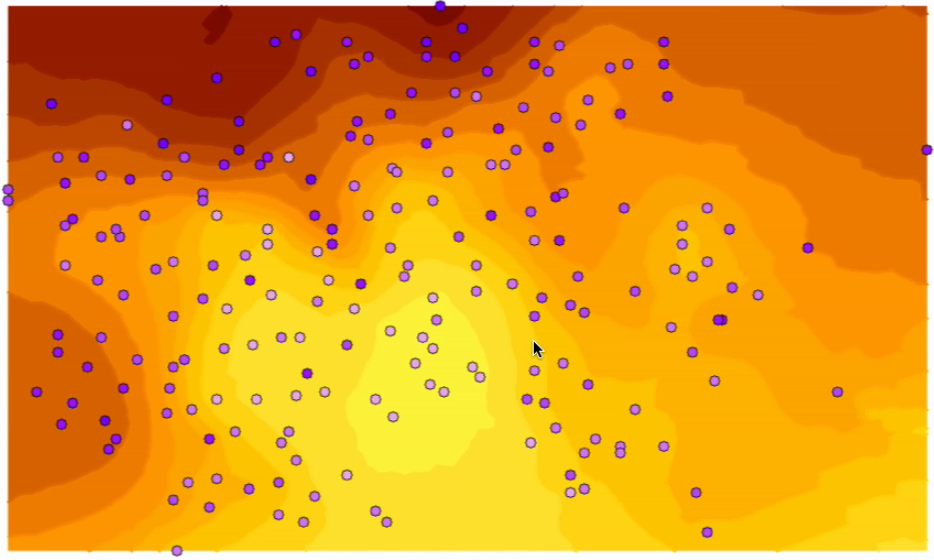
\includegraphics[width=1.00\linewidth]{baltimore.png}
    \end{center}
 \end{frame}


\begin{frame}[<+->]
  \frametitle{LA Basin Ozone Levels}
    \begin{center}
      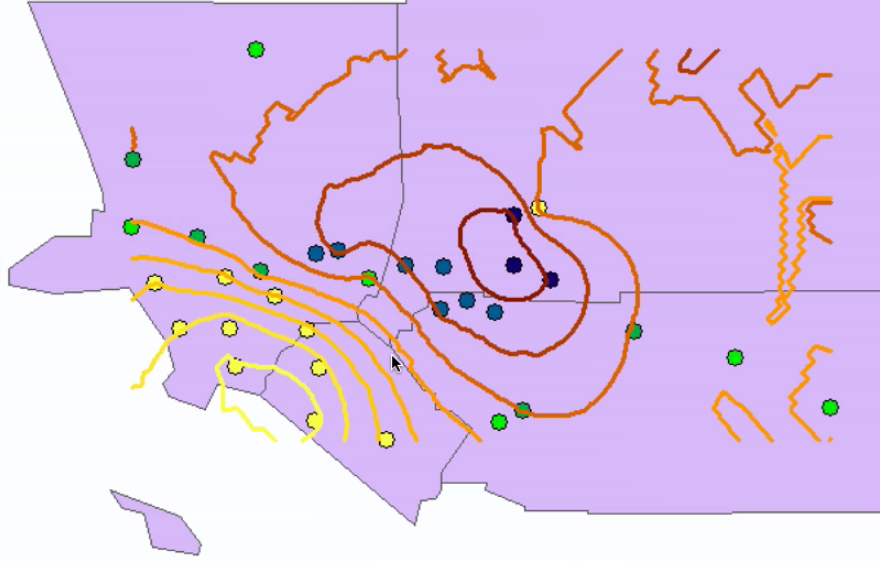
\includegraphics[width=1.00\linewidth]{laozone.png}
    \end{center}
 \end{frame}

 \begin{frame}
   \frametitle{Conceptual Framework}
   \begin{block}{Equilibrium}
     \begin{itemize}
       \item Equilibrium = Stationarity
       \item Stochastic Process
	 \begin{itemize}
	   \item not multiple realizations, but a single realization
	   \item the map is a single data point
	 \end{itemize}
       \item Notion of Stability
	 \begin{itemize}
	   \item go from a single data point to acting as if there are
	     multiple observations
	 \end{itemize}

     \end{itemize}
    \end{block}
  \end{frame}


\begin{frame}[<+->]
  \frametitle{Spatial Stationarity}
    \begin{center}
      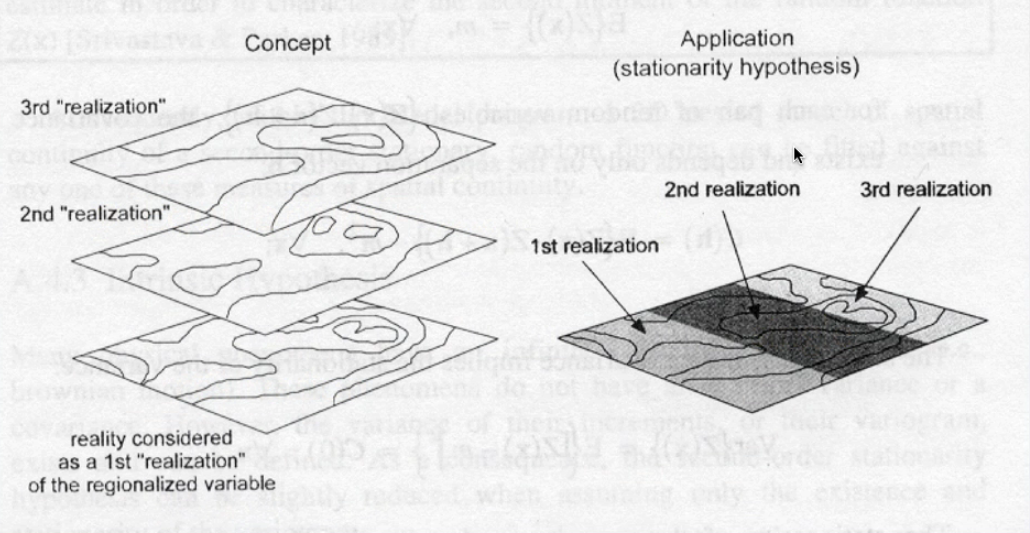
\includegraphics[width=1.00\linewidth]{variowin.png}
    \end{center}
 \end{frame}

 \begin{frame}
   \frametitle{Moment Conditions}
   \begin{itemize}
     \item Constrain Variability
     \item Moments Must Exist
       \begin{itemize}
	 \item no infinite variance
       \end{itemize}
     \item Moments Must Be Regular Over Space
   \begin{itemize}
     \item restrictions on heterogeneity
     \item restrictions on range of dependence
   \end{itemize}
   \end{itemize}
  \end{frame}

  \subsection{Moment Conditions}
  \begin{frame}
    \frametitle{Ergodicity}
    \begin{itemize}
      \item Sample Realization is Representative
	\begin{itemize}
	  \item average obtained using a single realization is same as over
	    all possible realizations
	  \item whether you observer one or many maps, the information should
	    be the same
	\end{itemize}
    \end{itemize}
   \end{frame}

   \begin{frame}
     \frametitle{Strict Stationarity}
     \begin{itemize}
       \item Pertains to the Complete Distribution
	\item Invariance Under Spatial Shift
	  \begin{itemize}
	    \item joint density for two different spatial subsets is same
	    \item $\{ z(s_l),\ldots,z(s_k)\}\ and\  \{
	      z(s_{l+h}),\ldots,z(s_{k+h})\}$
	    \item information about process is the same no matter where it is
	      obtained
	  \end{itemize}
	\item Very Strict Requirement
     \end{itemize}
    \end{frame}



   \begin{frame}
     \frametitle{Moment Stationarity}
     \begin{itemize}
       \item Moments Invariant Under Spatial Shift
	\item Mean
	  \begin{itemize}
	    \item no spatial trend
	  \end{itemize}
	\item Variance
	  \begin{itemize}
	    \item no heteroskedasticity (no spatial regimes)
	  \end{itemize}
	\item Covariance
	  \begin{itemize}
	    \item not a function of location
	    \item only spatial separation, angle
	  \end{itemize}
     \end{itemize}
    \end{frame}

\section{Variogram and Correlogram}
\begin{frame}
  \frametitle{Intrinsic Hypothesis}
  \begin{block}{No Spatial Trend}
    \begin{itemize}
  \item if there is a trend, take it out
  \item residuals have no trend (mean = 0
    \end{itemize}
   \end{block}
   \begin{block}{Constant Variance}
     \begin{itemize}
       \item Variance of first difference only a function of displacment
	 \begin{equation}
	   V \{Z_{s+h} - Z_s \}
	   \label{}
	 \end{equation}a
	 variability of the difference
     \end{itemize}
   \end{block}

 \end{frame}

\begin{frame}[<+->]
  \frametitle{Bubble Plot Baltimore House Sales Prices}
    \begin{center}
      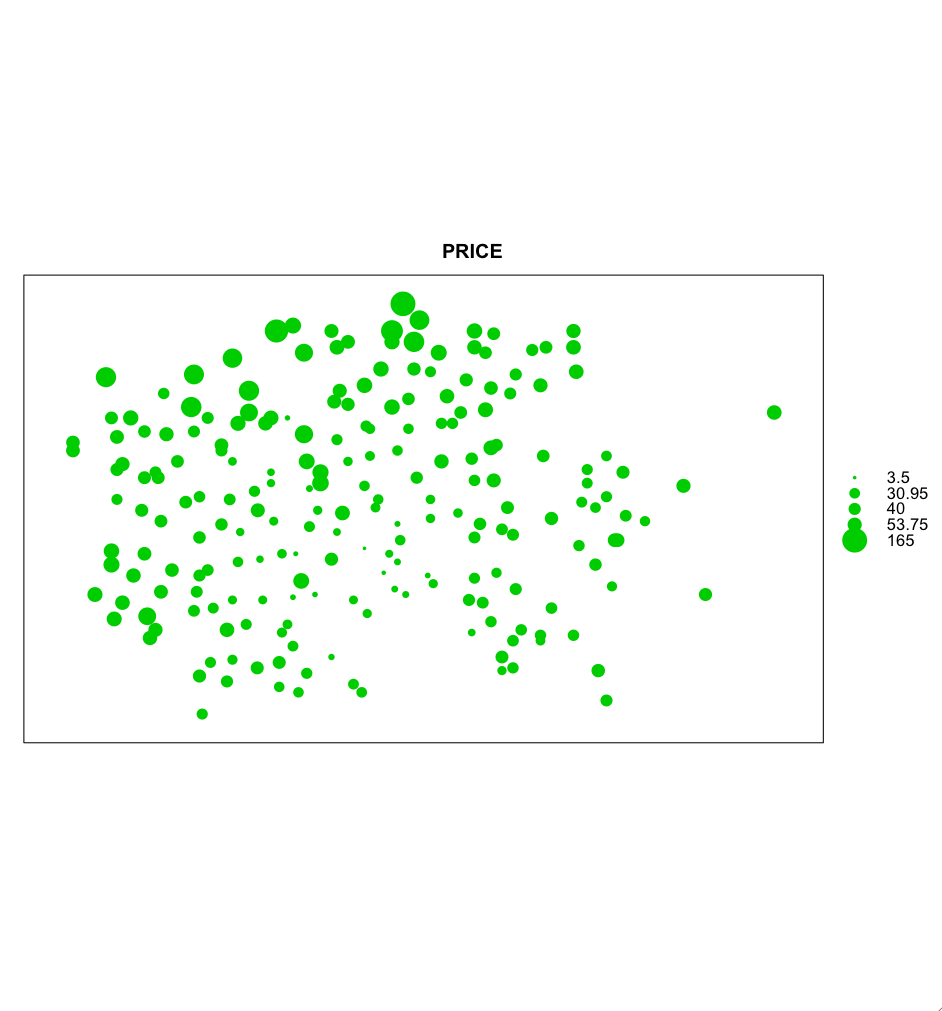
\includegraphics[width=0.8\linewidth]{bubble.png}
    \end{center}
 \end{frame}

\begin{frame}[<+->]
  \frametitle{Detrending Baltimore House Sales Prices}
    \begin{center}
      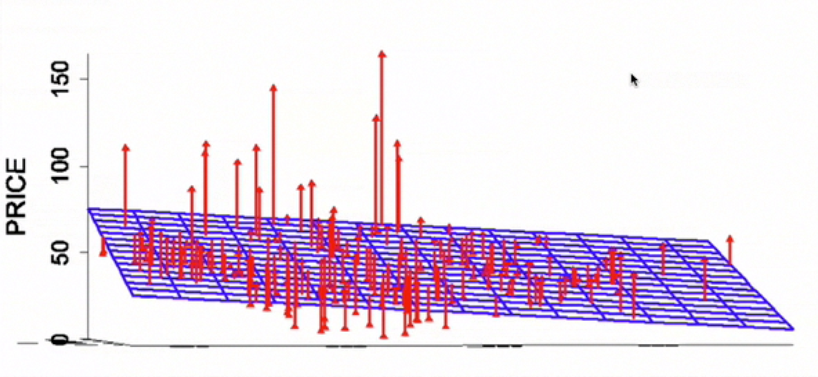
\includegraphics[width=1.00\linewidth]{baltimoretrend.png}

    $P=-166.02 - 0.148x + 0.634y$
    \end{center}
 \end{frame}
 \subsection{Semi-Variogram}
 \begin{frame}
   \frametitle{Semi-Variogram}
   \begin{block}{Variogram Function}
     \begin{equation}
       2 \gamma(h) = V [Z_{s+h} - Z_s ]
     \end{equation}
     factor 2, so $\gamma(h)$ is half of the variogram, or semi-variogram
    \end{block}
    \begin{block}{Constant Mean Assumption}
      \begin{itemize}
	\item $E[Z_{s+h} - Z_s] = E[Z_{s+h}] - E[Z_s] = 0$
	\item $V[Z_{s+h} - Z_s] = E[Z_{s+h} - E[Z_s]]^2 - 0$
	\item $\gamma(h) = (1/2) E[Z_{s+h} - E[Z_s]]^2$
	\item average of squared differences
      \end{itemize}

    \end{block}
  \end{frame}

\begin{frame}[<+->]
  \frametitle{Variogram Cloud}
    \begin{center}
      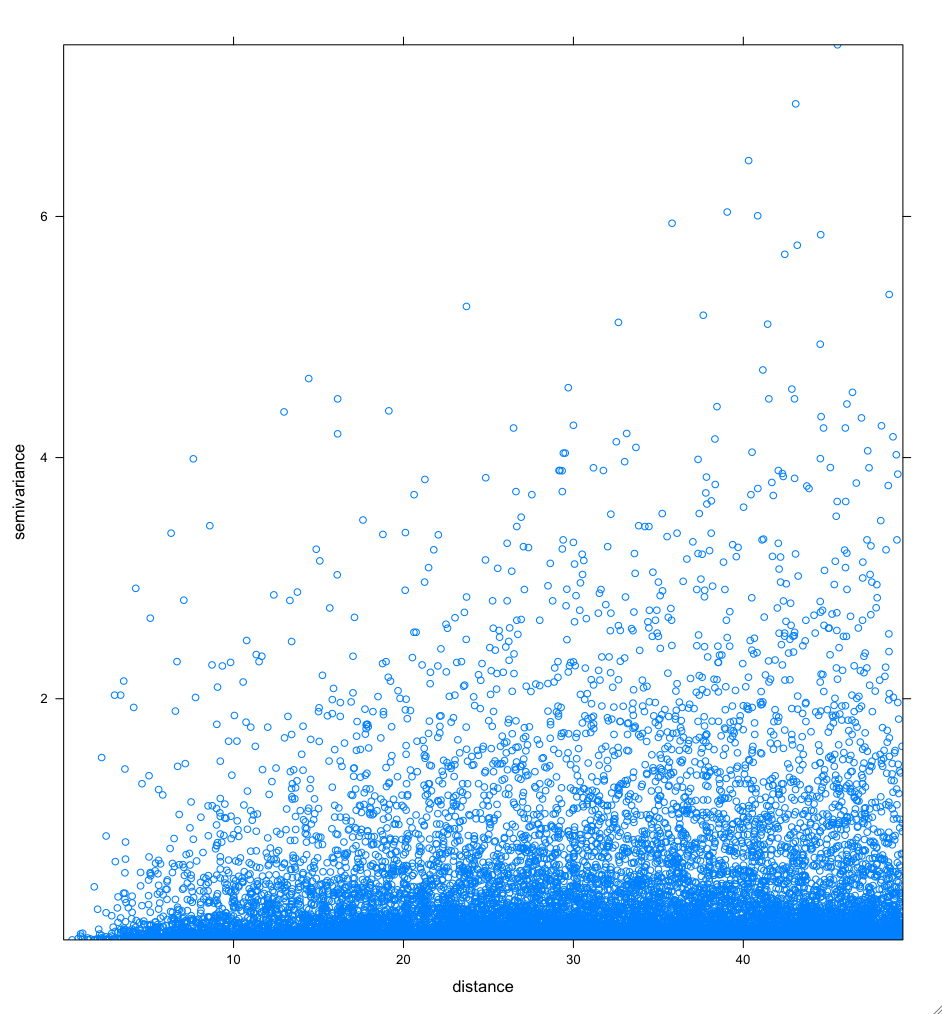
\includegraphics[width=0.60\linewidth]{cloud.png}
    \end{center}
 \end{frame}

\begin{frame}[<+->]
  \frametitle{Outliers in Variogram Cloud}
    \begin{center}
      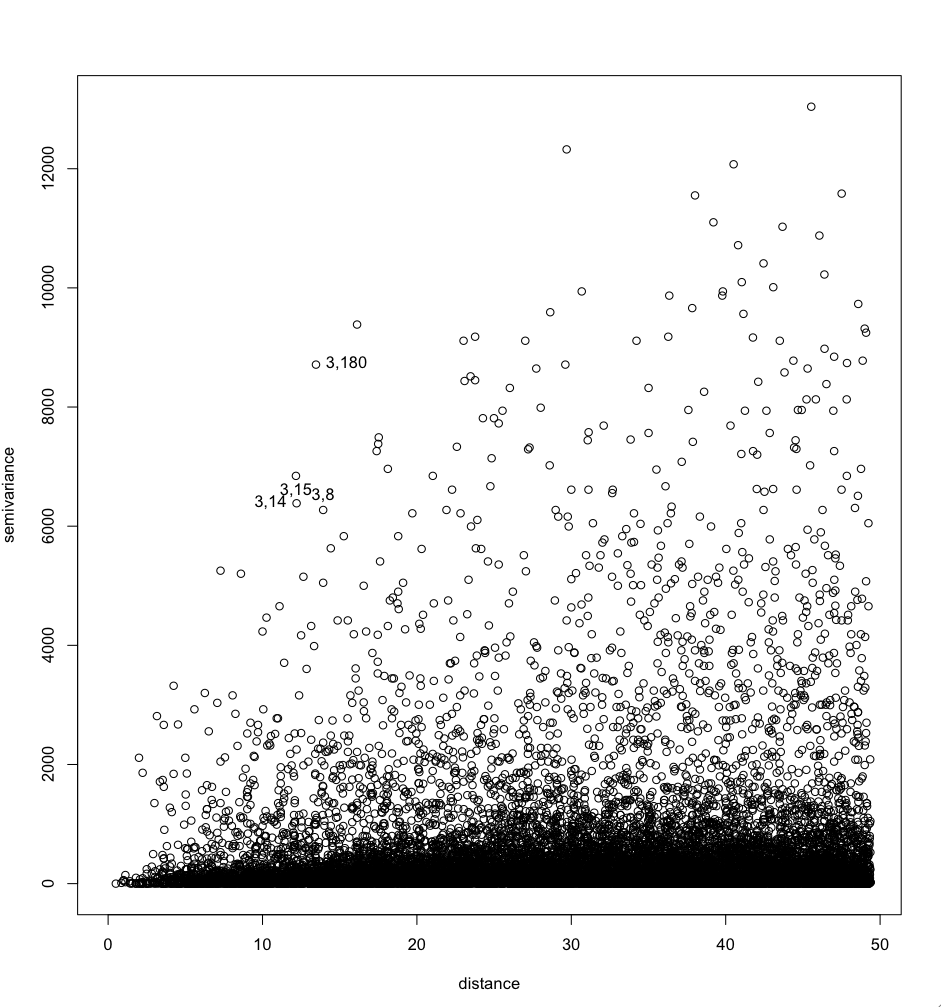
\includegraphics[width=0.60\linewidth]{cloudoutlier.png}
    \end{center}
 \end{frame}


\begin{frame}[<+->]
  \frametitle{Outliers in Bubble Plot}
    \begin{center}
      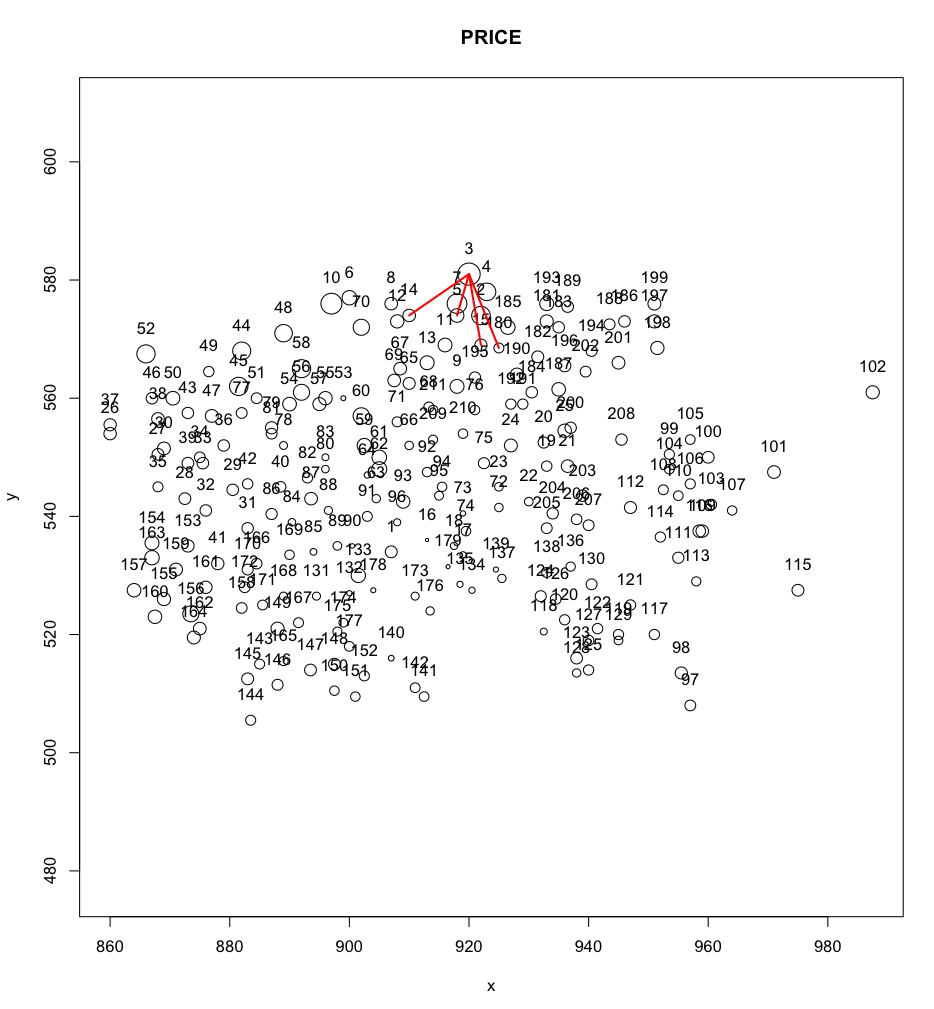
\includegraphics[width=0.60\linewidth]{bubbleoutlier.png}
    \end{center}
 \end{frame}

 \begin{frame}
   \frametitle{Estimating a Variogram}
   \begin{block}{Methods of Moments}
     \begin{equation}
       2\gamma(h) = (1 / |N(h)|) \sum_h [Z_{s+h} - Z_s]^2
       \label{}
     \end{equation}
       \begin{itemize}
	 \item average of squared differences by distance bin $h$
	 \item $N(h)$ number of pairs in distance bin $h$
       \end{itemize}
    \end{block}
    \begin{block}{Rules of Thumb}
      \begin{itemize}
	\item at least 30 pairs in each bin
	\item max $h < D/2$ ($D$ is maximum distance)
	\item distance of reliability
      \end{itemize}
    \end{block}
  \end{frame}

\begin{frame}[<+->]
  \frametitle{Variogram on 2nd Order Trend Surface}
    \begin{center}
      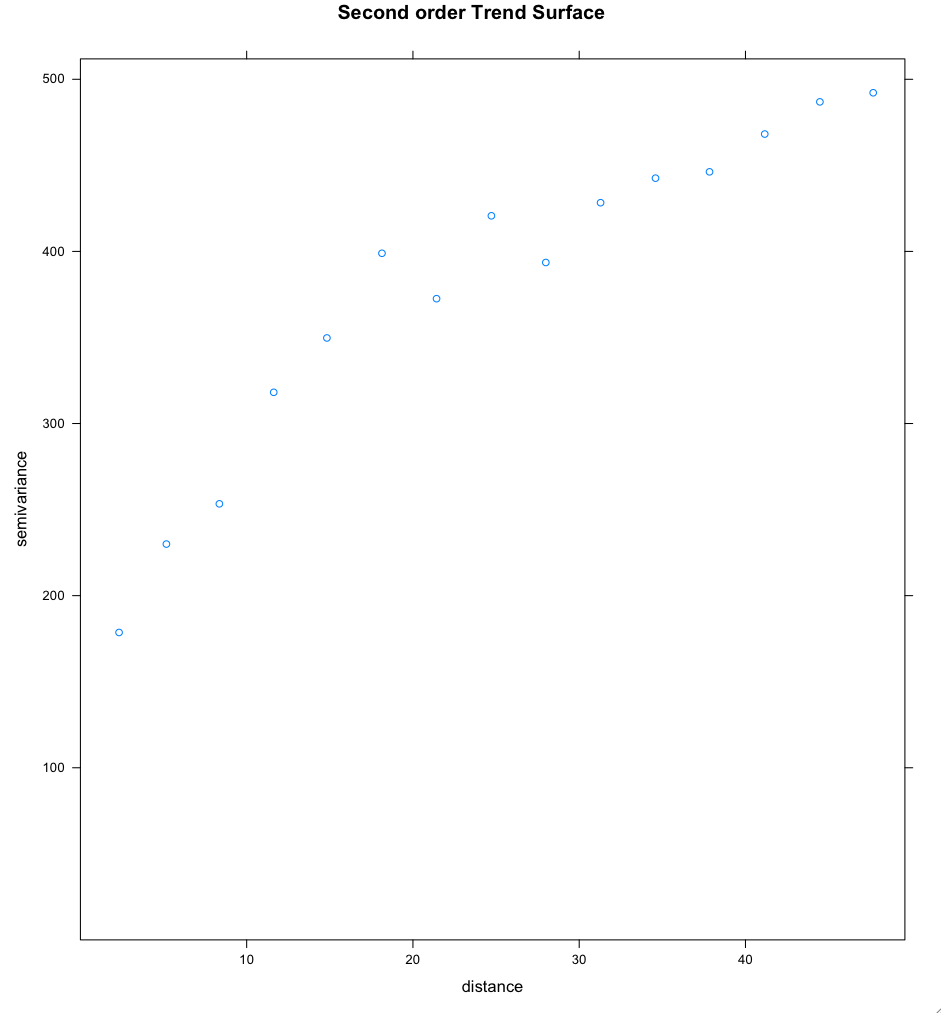
\includegraphics[width=0.60\linewidth]{variogram2d.png}
    \end{center}
 \end{frame}
 \subsection{Covariogram}
 \begin{frame}
   \frametitle{Covariogram}
   \begin{block}{Second Order Stationarity}
     \begin{itemize}
       \item covariance regular over space
       \item stronger assumptions: regularity second order moments,
	 cross-product
     \end{itemize}
    \end{block}
    \begin{block}{Covariance at $h$}
      \begin{equation}
	C(h) = Cov[Z_{s+h},Z_s]
	\label{}
      \end{equation}
    \end{block}
    \begin{block}{Process Variance}
      \begin{itemize}
	\item covariance at distance zero
	\item $C(0) = V[Z_s]$
      \end{itemize}
    \end{block}

  \end{frame}

  \begin{frame}
    \frametitle{Correlogram}
    \begin{block}{Autocorrelation Function}
      \begin{equation}
	\rho(h) = C(h)/C(0)
	\label{}
      \end{equation}
      covariance standardized by proces variance
     \end{block}
     \begin{block}{ Distance Decay}
       \begin{itemize}
	 \item Correlogram decreases with distance
	 \item Tobler's law
       \end{itemize}
     \end{block}
   \end{frame}
   \begin{frame}
     \frametitle{Semi-Variogram and Covariogram}
     \begin{block}{Two approaches to same concept}
       \begin{eqnarray}
	 2\gamma(h)& =& E[Z_{s+h} - Z_s]^2 \\
	 &=&2 E[Z_s^2] - 2 E[Z_{s+h}Z_s]
       \end{eqnarray}
      \end{block}
      \begin{block}{Semi-variance}
	\begin{itemize}
	  \item $\gamma(h) = C(0) - C(h)$
	  \item semi-variance is variance of process less covariance at
	    distance $h$
	\end{itemize}

      \end{block}
    \end{frame}
\begin{comment}
\subsection{Quadrat Test Example}

  \begin{frame}[containsverbatim]
    \frametitle{Code: ihhpsim.r}
    \begin{small}
      \begin{verbatim}
source("quadcounts.r")
source("ihppsim.r")
pp=ippsim(100)*9+1
ppt=quadcount(pp[,1],pp[,2])
set.seed(100)
nsim=99
source("hppsim.r")
results=matrix(0,nsim+1,1)
for(i in 1:nsim){
    pp=csr(100,1,1,10,10)
    t=quadcount(pp$x,pp$y)
    results[i]=t$chi2
}
results[100]=ppt$chi2
plot(density(results),main="Quadrat Test of Inhomogenous Poisson
Point Process",xlab="Chi^2",ylab="f(Chi^2)")
abline(v=ppt$chi2,col='red')
      \end{verbatim}
    \end{small}
   \end{frame}



\begin{frame}[<+->] 
    \frametitle{Empirical Sampling Distribution}
    \begin{center}
      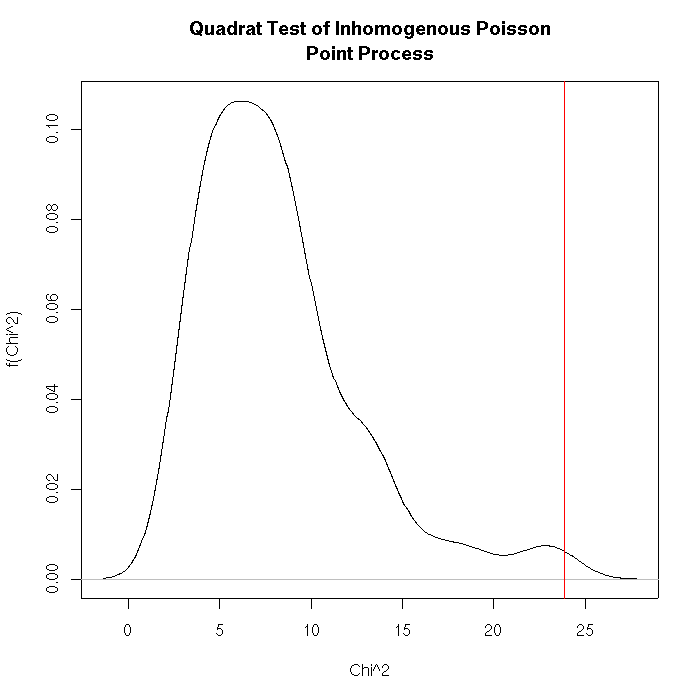
\includegraphics[width=.65\linewidth]{mcsim.png}
    \end{center}
  \end{frame}

\begin{frame}[<+->]
    \frametitle{Pseudo Significance Level}
    \begin{block}{p-value}
      \begin{equation}
	p(\chi^2) = \frac{1+ \sum_{i=1}^{nsim} \psi_i}{nsim+1}
      \end{equation}
      where:
      \begin{equation}
	\psi_{i} = \left\{ \begin{array}{ll}
	  1& if \ \chi_i^2 \ge \chi^2, \\
	  0&otherwise\\
	\end{array} \right.
      \end{equation}
     \end{block}
\begin{block}{p-value}
      \begin{equation}
	\hat{p(\chi^2)} = \frac{1+ 0}{99+1} = 0.01
      \end{equation}
     \end{block}
  \end{frame}


\section{Nearest Neighbor Distance Methods}
\subsection{Mean Nearest Neighbor Statistic}
\begin{frame}[<+->]
  \frametitle{Mean Nearest Neighbor Statistic}
  \begin{block}{$d_{min}(s_i)$}
    \begin{equation}
      d_{min}(s_i) = min(d_{i,1},d_{i,2},\ldots,d_{i,n})
    \end{equation}
   $d_{min}(s_i)$ is the distance between $i$ and its nearest neighbor event.
   \end{block}
  \begin{block}{Test Statistic}
    \begin{equation}
	\bar{d}_{min}= \frac{1}{n} \sum_{i=1}^n d_{min}(s_i)
    \end{equation}
    Originally suggested by Clark and Evans (1954)
   \end{block}
 \end{frame}
\begin{frame}[<+->]
  \frametitle{Mean Nearest Neighbor Statistic Distribution}
  \begin{block}{$\bar{d}_{min}^{\sim}N(\mu,\sigma^2)$}
    \begin{equation}
      \mu=E[\bar{d}_{min}] = 0.5(n^{-1} |A|)^{1/2} + (0.051 + 0.042n^{-1/2})n^{-1}
      P
    \end{equation}
    \begin{equation}
      \sigma^2 = V[\bar{d}_{min}] =0.070n^{-1/2} |A| + 0.037(n^{-5}|A|)^{1/2}P
    \end{equation}
    where $|A|$ and $P$ are the area and perimeter of the study area,
    respectively.
   \end{block}
   \begin{block}{Issues}
     \begin{itemize}
       \item Approximation, not an exact result.
       \item Dependence of nearest neighbor distances is ignored.
       \item Distribution of $d_{min}(s_i)$ ignored (only first moment).
     \end{itemize}
   \end{block}
 \end{frame}


\subsection{Nearest Event-Event Neighbor Distance Functions}

\begin{frame}[<+->]
    \frametitle{Nearest Neighbor G Function}
    \begin{block}{$G(d)$}
      \begin{equation}
	G(d) = \sum_{i=1}^n \Phi_{i}^d / n
      \end{equation}
      where
\begin{equation}
	\Phi_{i}^d = \left\{ \begin{array}{ll}
	  1& if \ d_{min}(s_i) < d \\
	  0&otherwise\\
	\end{array} \right.
      \end{equation}
      $G(d)$ is the proportion of nearest neighbor distances that are less
      than $d$.
    \end{block}
  \end{frame}

\begin{frame}[<+->]
    \frametitle{Uganda Crater Data}
    \begin{center}
      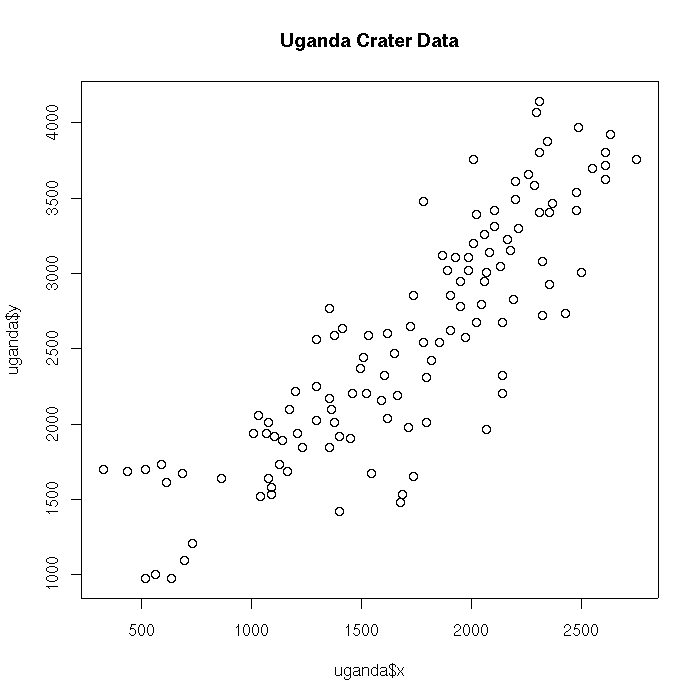
\includegraphics[width=.65\linewidth]{uganda.png}
    \end{center}
  \end{frame}


\begin{frame}[<+->]
    \frametitle{Nearest Neighbor G Function}
    \begin{center}
      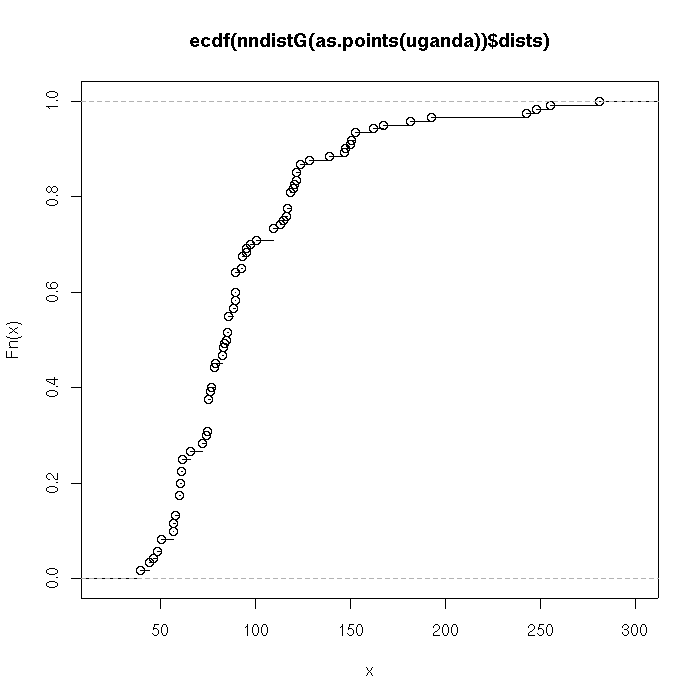
\includegraphics[width=.65\linewidth]{nng.png}
    \end{center}
  \end{frame}
  \begin{frame}[<+->]

    \frametitle{G Function Intepretation}
    \begin{block}{Shape}
      \begin{itemize}
	\item G increasing rapidly at small distances points to
	  \emph{clustering}.
	\item G increases slowly points to \emph{uniformity}.
	\item Both are deviations from CSR.
      \end{itemize}
     \end{block}
\begin{block}{Compare G to that from a CSR Process}
      \begin{itemize}
	\item Theoretical G
	    \item Homogeneous Poisson process
	    \item Density equal to density of actual pattern
	\item Empirical distribution against theoretical distribution
	  \begin{itemize}
	    \item Should be a 45 degree line if process is CSR
	    \item Above the line = clustering
	    \item Below the line = dispersion
	  \end{itemize}
      \end{itemize}
     \end{block}


   \end{frame}

\begin{frame}[<+->]
    \frametitle{Estimated vs. Theoretical G Function}
    \begin{center}
      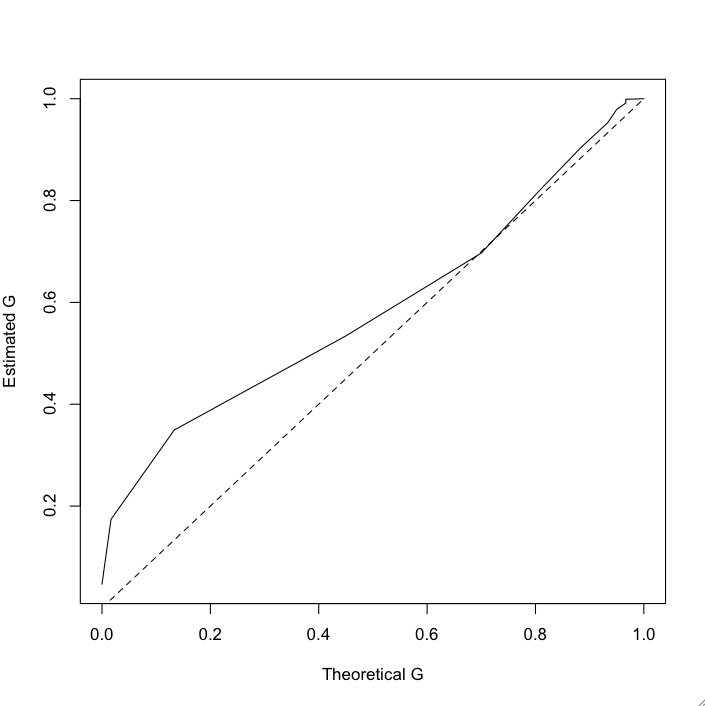
\includegraphics[width=.65\linewidth]{theoryg.png}
    \end{center}
  \end{frame}



  \begin{frame}[containsverbatim]
    \frametitle{Estimated vs. Theoretical G Function: Code}
    \begin{small}
      \begin{verbatim}
> data(uganda)
> plot(Ghat(as.points(uganda), seq(20, 500, 20)),
+ Fzero(pdense(as.points(uganda),  uganda$poly),
+ seq(20, 500, 20)), type="l", 
+ ylab="Theoretical G", 
+ xlab="Estimated G")
> lines(c(0,1),c(0,1),lty=2)
      \end{verbatim}
    \end{small}
   \end{frame}


\begin{frame}[<+->]
    \frametitle{Nearest Neighbor G Function}
    \begin{center}
      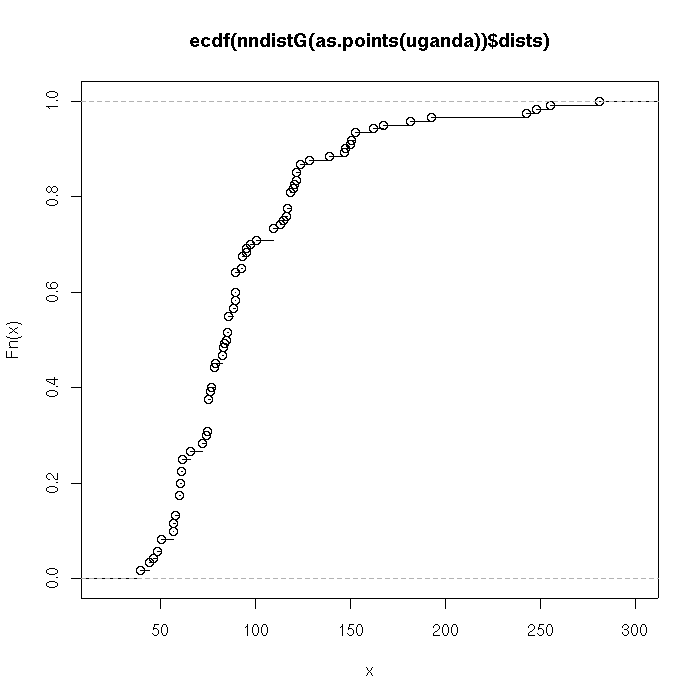
\includegraphics[width=.65\linewidth]{nng.png}
    \end{center}
  \end{frame}


\subsection{Nearest Point-Event Neighbor Distances}

\begin{frame}[<+->]
    \frametitle{Nearest Neighbor F Function}
    \begin{itemize}
      \item G function is sensitive to $n$
	\begin{itemize}
	  \item Can be rough
	  \item Takes on stepped appearance for small $n$
	\end{itemize}
      \item Alternative approach is to generate $N$ random points in the
	domain
	\begin{itemize}
	  \item Analyze the distribution of nearest event neighbor distances
	  \item Closest event to each point.
	\end{itemize}
      \item Can be used for small $n$ data sets
    \end{itemize}
  \end{frame}


\begin{frame}[<+->]
    \frametitle{Nearest Neighbor F Function}
    \begin{center}
      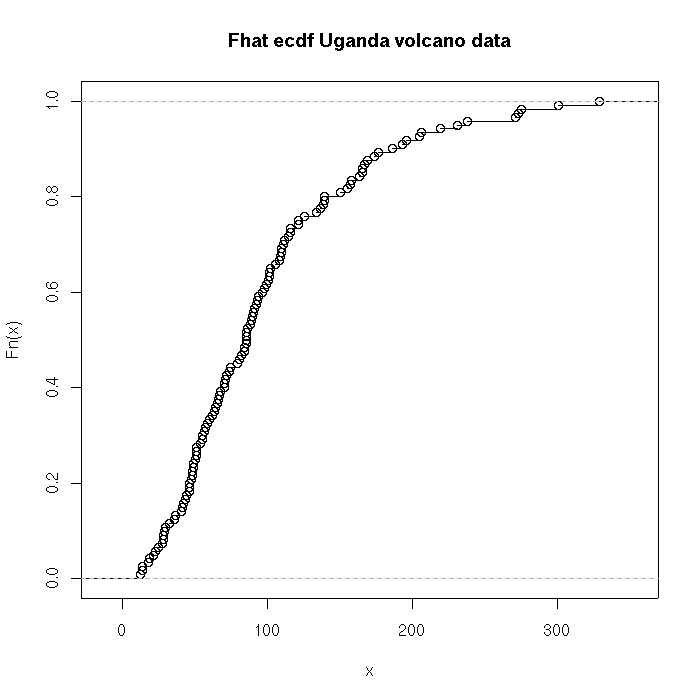
\includegraphics[width=.65\linewidth]{nnf.png}
    \end{center}
  \end{frame}

 \section{Inter-Event Distance Distributions}
 \begin{frame}[<+->]
   \frametitle{Inter-Event Distance Distributions}
   \begin{block}{$G$ and $F$ Functions}
     \begin{itemize}
       \item Take account of the nearest neighbor distributions: $n$ distances
	 or pieces of
	 information
       \item Do not account for the full distribution of inter-event distances
	 $n(n-1)/2$ distances.
     \end{itemize}
\end{block}
     \begin{block}{Inter-Event Distances}
       \begin{itemize}
	 \item Consider all inter-event distances
	 \item More than one distance for each point
	 \item Second order analysis
	   \begin{itemize}
	     \item Expresses the dependence of events
	     \item Spatial interaction
	   \end{itemize}
       \end{itemize}
     \end{block}
  \end{frame}

  \begin{frame}[<+->]
    \frametitle{Ripley's $K$ function}
    \begin{block}{$K$}
      \begin{equation}
	K(d) = \frac{\sum_{i=1}^n \sum_{j=1}^n \psi_{ij}(d)}{n\lambda}
      \end{equation}
where:
      \begin{equation}
	\psi_{ij}(d) = \left\{ \begin{array}{ll}
	  1& if \ d_{ij} \le d \\
	  0&otherwise\\
	\end{array} \right.
      \end{equation}

     \end{block}
     \begin{block}{Circle centered on each point $s_i$}
       \begin{equation}
	 \sum_{j=1}^n \psi_{ij}(d)
       \end{equation}
       is the number of events within a circle of radius $d$ centered on even
       $s_i$.
     \end{block}
   \end{frame}


\begin{frame}[<+->]
    \frametitle{Point Pattern Example}
    \begin{center}
      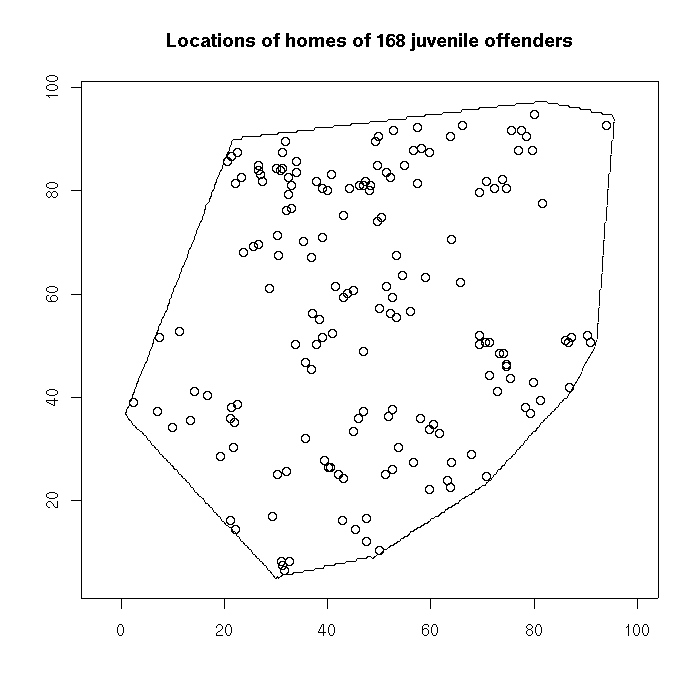
\includegraphics[width=.65\linewidth]{splancs.png}
    \end{center}
  \end{frame}

\begin{frame}[<+->]
    \frametitle{K function}
    \begin{center}
      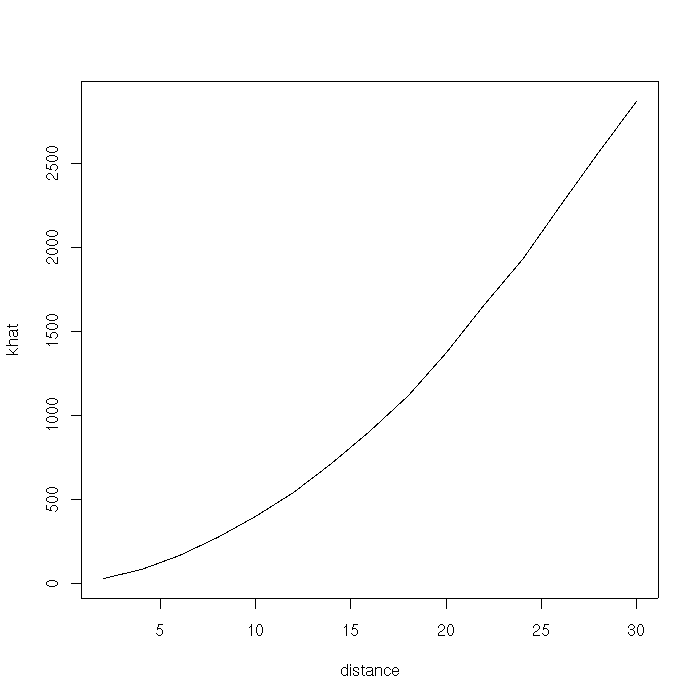
\includegraphics[width=.65\linewidth]{kfunction.png}
    \end{center}
  \end{frame}
 


  \begin{frame}[containsverbatim]
    \frametitle{Splancs K function simulation}
    \begin{small}
      \begin{verbatim}
> UL.khat <- Kenv.csr(length(cardiff$x), cardiff$poly,
+ nsim=29, seq(2,30,2))
Doing simulation  1 
Doing simulation  2 
.
Doing simulation  28 
Doing simulation  29 
> plot(seq(2,30,2), sqrt(khat(as.points(cardiff),
+ cardiff$poly, 
+ seq(2,30,2))/pi)-seq(2,30,2), type="l", xlab="Distance", 
+ ylab="Estimated L", ylim=c(-1,1.5))
> lines(seq(2,30,2), sqrt(UL.khat$lower/pi)-seq(2,30,2),
+ lty=2)
> lines(seq(2,30,2), sqrt(UL.khat$upper/pi)-seq(2,30,2),
+ lty=2)
      \end{verbatim}
    \end{small}
   \end{frame}

\begin{frame}[<+->]
    \frametitle{K function simulation}
    \begin{center}
      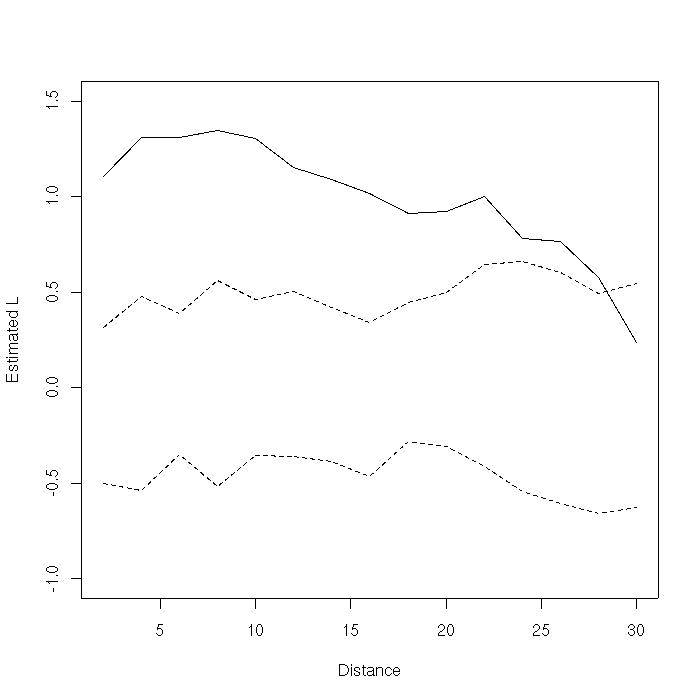
\includegraphics[width=.65\linewidth]{kfunctionsim.png}
    \end{center}
  \end{frame}

\begin{frame}[<+->]
    \frametitle{$L$ function}
    \begin{block}{Scaling of $K$}
      \begin{equation}
	L(d) = \sqrt{ K(d)/\pi } - d
      \end{equation}
    \end{block}
    \begin{block}{ Useful since:}
    \begin{equation}
      E[K(d)] = \frac{\pi \lambda d^2}{\lambda}
    \end{equation}
    which can get large with $d^2$ and obscures small differences between
    expected and observed values.
  \end{block}
  \end{frame}
 

  \begin{frame}[<+->]
    \frametitle{Edge Effects}
    \begin{block}{Problems}
      \begin{itemize}
	\item For points close the the boundary intensity is underestimated.
	\item Neighboring points are outside the study region.
      \end{itemize}
\end{block}
      \begin{block}{Solutions}
	\begin{itemize}
	  \item Buffer the points
	  \item Edge corrections
	  \item Monte Carlo Simulations
	\end{itemize}
      \end{block}
   \end{frame}
 \end{comment}
\end{document}
